\chapter{Data Pre-processing}
Nella realtà, i dati che vengono utilizzati per effettuare le varie analisi non
sono mai perfetti, anzi, sono spesso ``sporchi'', ovvero possono essere:
\begin{itemize}
      \item \textbf{Incompleti}: ovvero mancano valori per alcune feature.
      \item \textbf{Rumorosi}: ovvero contengono errori e/o outlier.
      \item \textbf{Inconsistenti}: sono presenti discrepanze nei dati.
\end{itemize}
Quando nei dati che si vogliono utilizzare per la creazione di un modello siamo
in presenza di queste condizioni, allora si devono compiere i seguenti passaggi:
\begin{enumerate}
      \item \textbf{Data cleaning}: in questa fase si vanno a risolvere i vari
            problemi di incompletezza, rumorosità e inconsistenza dei dati.
      \item \textbf{Data integration}: i dati possono essere presenti in più
            dataset, quindi si devono integrare insieme.
      \item \textbf{Data transformation}: in questa fase si vanno ad applicare
            operazioni di normalizzazione e aggregazione dei dati.
      \item \textbf{Data reduction}: selezione delle feature ed estrazione di
            sottoinsiemi di esse.
\end{enumerate}
\section{Data cleaning}
\subsection{Valori mancanti}
\begin{definizione} [\textbf{Valori mancanti}]
      Possiamo definire i \textbf{valori mancanti} come valori sconosciuti di una
      feature per una particolare istanza.
\end{definizione}
La presenza dei \textbf{valori mancanti} può essere dovuta a diversi fattori,
tra cui:
\begin{itemize}
      \item Dati non disponibili
      \item Dati non registrati
      \item Risultati di malfunzionamenti dei sensori
      \item Dati cancellati
      \item Dati sconosciuti
\end{itemize}
La gestione di valori mancanti è un problema molto importante ed è necessario
gestirli in modo corretto. La loro gestione è importante per le seguenti ragioni:
\begin{itemize}
      \item \textbf{Perdita di efficienza}: rendono meno efficienti i processi che
            vengono successivamente applicati ai dati. Inoltre la loro presenza può
            influenzare i risultati in quanto introduciamo delle distorsioni nel
            dataset.
      \item \textbf{Complicazioni}: si complicano i modelli perché non prevedono
            valori mancanti nelle istanze. Esistono modelli che sono in grado di
            superare questo problema ma sono più complessi.
      \item \textbf{Bias nei risultati}: si introducono delle differenze tra dati
            completi e dati incompleti.
\end{itemize}

Esistono 3 tipologie di dati mancanti:
\begin{itemize}
      \item \textbf{Missing Completely At Random} (\textbf{MCAR}): quando la
            mancanza del valore di un attributo è randomica e non è dipendente dai valori
            osservati o dai valori mancanti.
      \item \textbf{Missing At Random} (\textbf{MAR}): quando la mancanza del
            valore di un attributo è dipendente dai valori osservati, ma non dai
            valori mancanti.
      \item \textbf{Not Missing At Random} (\textbf{NMAR}): quando la mancanza del
            valore di un attributo è dipendente dai valori mancanti.
\end{itemize}
In base alla tipologia del dato mancante si hanno diversi metodi per la loro
gestione di essi. I principali metodi sono i seguenti:
\begin{itemize}
      \item \textbf{Ignorare} l'istanza avente il valore dell'attributo mancante o
            ignorare l'attributo se molte istanze hanno valori mancanti per quella
            feature. Questo è l'approccio più semplice ma applicabile solo quando
            abbiamo pochi dati mancati rispetto a quelli dati osservati.
      \item \textbf{Conversione} dei valori mancanti. Si assegna un significato al
            valore mancante, quindi, in termini di modelli probabilistici, si
            aggiunge un ulteriore possibile valore alla variabile aleatoria e
            \textit{si considera come un'informazione} il fatto che manchi il valore.
      \item \textbf{Metodi di imputazione}, assegno un valore basato sul resto delle
            osservazioni del dataset, ma non è importate sapere che manchi e quindi
            meglio un valore che lo sostituisca. Questo metodo è applicabile per i
            dati di tipo \textit{MCAR} e \textit{MAR}, ma non per \textit{NMAR}.
\end{itemize}
\subsubsection{Metodi di imputazione}
A seconda della situazione e in base alla tipologia dell'attributo, si possono
usare diversi metodi di imputazione dei valori mancanti:
\begin{itemize}
      \item Una prima strategia è quella \textbf{most common value}, la quale
            fornisce due possibilità di imputazione:
            \begin{itemize}
                  \item \textbf{Continuo}: calcolo la media tra tutti gli altri
                        valori delle features, in questa situazione si assume che il
                        dato sia distribuito normalmente.
                  \item \textbf{Discreto} o \textbf{Categorico}: sostituiamo il valore
                        mancante con quello più frequente.
            \end{itemize}
      \item Un'altra strategia è quella \textbf{concept most common value}, la
            quale utilizza le stesse strategie di imputazione ma in base alla 
            classe dell'istanza.
\end{itemize}
Il primo approccio si può utilizzare in un contesto non supervisionato, mentre il
secondo in un contesto supervisionato. Inoltre il primo approccio assume che tutti
gli attributi siano distribuiti normalmente, mentre il secondo assume che le
distribuzioni degli attributi della stessa classe derivino da una normale.

Gli approcci appena descritti sono molto semplici e veloci, ne esistono altri più
complessi che scomodano algoritmi di Machine Learning. Per esempio si può usare
\textbf{kNN} per predire il valore mancante in base al valore più frequente tra
i $k$ valori degli esempi più vicini. Un estensione di questo metodo è l'utilizzo
di algoritmi di Machine Learning per la predizione dei valori mancanti. Questo
significa definire un modello per la previsione dei valori mancanti per ciascuna
feature, il che lo rende computazionalmente molto costoso.

\subsection{Rumorosità dei dati}
\begin{definizione} [\textbf{Rumorosità dei dati}]
      La \textbf{Rumorosità dei dati} è l'insieme di dati che presentano dei
      valori che non hanno una relazione con gli altri valori, spesso dovuti ad
      errori di misurazione o errori nella scelta del campione.
\end{definizione}
Una possibilità per ridurre il rumore consiste nel discretizzare (\textbf{Binning})
i dati continui attraverso i seguenti metodi:
\begin{itemize}
      \item \textbf{Equal-width}: partiziona dell'intervallo dell'attributo in $N$
            intervalli della stessa larghezza. Mantiene sempre gli outliers e
            quindi la distribuzione non è uniforme.
            Ad esempio se abbiamo un intervallo $[0, 100]$ e vogliamo partizionarlo
            in 5 intervalli, otteniamo $[0, 20]$, $[20, 40]$, $[40, 60]$, $[60, 80]$,
            $[80, 100]$.

            \begin{figure}[!ht]
                  \centering
                  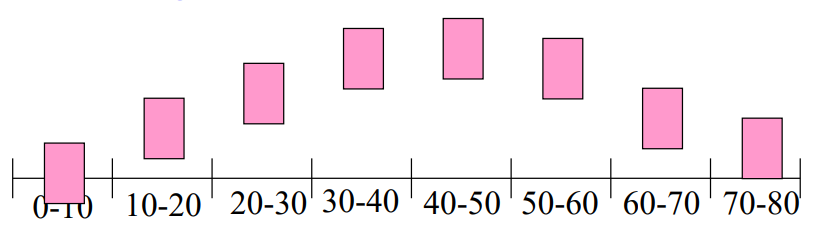
\includegraphics[width=0.7\textwidth]{./img/Preprocessing/equalwidth.png}
                  \caption{Equal-width}
                  \label{fig:equal-width}
            \end{figure}

      \item \textbf{Equal-depth}: partiziona dell'intervallo dell'attributo in $N$
            intervalli in cui la frequenza dei dati è la stessa. Genera una
            distribuzione uniforme ma non mantiene gli outliers. Si riduce la
            varianza.

            \begin{figure}[!ht]
                  \centering
                  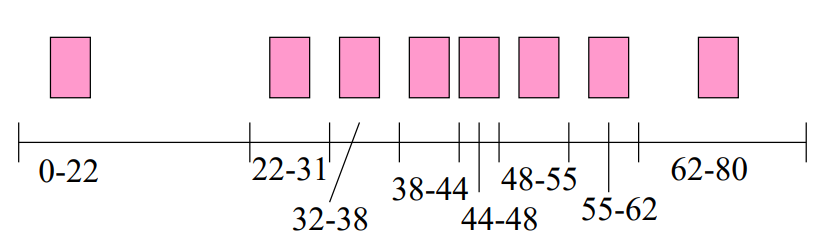
\includegraphics[width=0.7\textwidth]{./img/Preprocessing/equaldepth.png}
                  \caption{Equal-width}
                  \label{fig:equal-depth}
            \end{figure}
\end{itemize}
Entrambi i modelli hanno lo scopo di ridurre la varianza dei dati, in quanto si
sta passando da uno spazio continuo a uno spazio discreto. La differenza tra i
due metodi è che il primo mantiene gli outliers, mentre il secondo no.
\subsection{Dataset sbilanaciato}
Parliamo di \textbf{dataset sbilanciato} quando le classi di un dataset non sono
rappresentate dalla stessa frequenza. Nello specifico questa situazione si
verifica quando una classe sovrasta completamente l'altra. Ad esempio se abbiamo
un dataset in cui l'$80\%$ delle istanze appartiene alla classe $A$ e il restante
$20\%$ alla classe $B$, allora il dataset è sbilanciato.

È importante osservare che quando si parla di sbilanciamento del dataset
non bisogna considerare solamente la frequenza. Infatti, sebbene una classe
possa essere rappresentata da un numero maggiore di istanze, queste potrebbero
essere linearmente separabili, quindi non si hanno problemi dal punto di vista
di algoritmi che cercano una frontiera di separazione.

Al contrario, per un metodo di classificazione come \textbf{Bayes} in cui la
dimensione del campione è importante, avere un dataset sbilanciato può portare
a risultati errati.

Una possibile soluzione consiste nel bilanciare il dataset, ovvero cercare di
rendere le classi rappresentate da un numero simile di istanze. Questo può essere
fatto attraverso due metodi:
\begin{itemize}
      \item \textbf{Oversampling}: consiste nel duplicare le istanze della classe
            meno rappresentata.
      \item \textbf{Undersampling}: consiste nel rimuovere le istanze della classe
            più rappresentata.
\end{itemize}
\begin{nota}
      Quando si effettua un oversempling bisogna stare attenti in quanto si
      potrebbero introdurre delle distorsioni nel dataset.
\end{nota}
Vediamo ora un esempio di algoritmo che mi permette di effettuare l'oversempling
del dataset. Tale algoritmo è chiamato \textbf{SMOTE} (\textbf{Synthetic Minority
      Over-sampling Technique}). Questo algoritmo funziona nel seguente modo:
\begin{enumerate}
      \item Si seleziona un'istanza della classe meno rappresentata.
      \item Partendo da questa, attraverso un algoritmo di \textbf{kNN}, si
            selezionano le $k$ istanze più vicine.
      \item Si seleziona un sottoinsieme casuale di queste istanze e si calcola la
            la media tra queste.
      \item Si aggiunge questa nuova istanza al dataset.
      \item Si ripete il procedimento fino a quando non si raggiunge un numero
            sufficiente di istanze.
\end{enumerate}
\begin{figure}[!ht]
      \centering
      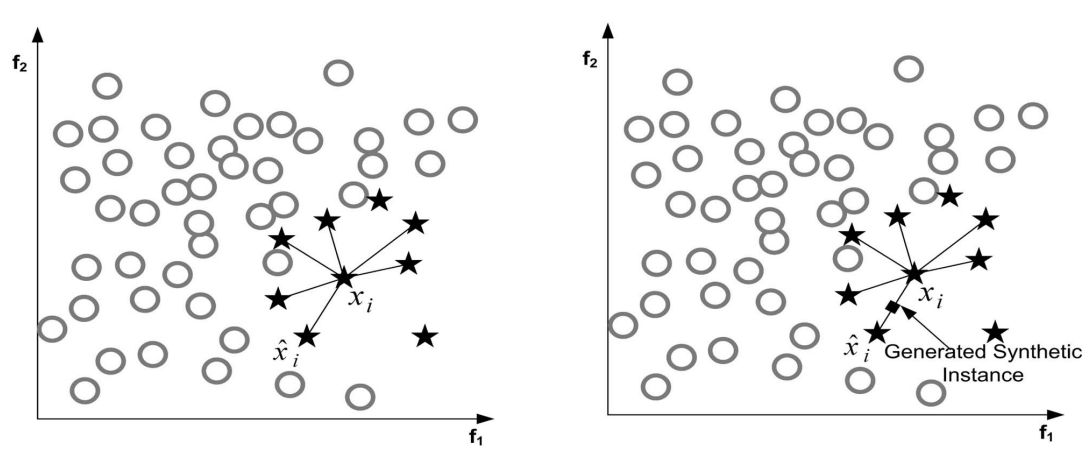
\includegraphics[width=0.5\textwidth]{./img/Preprocessing/smote.png}
      \caption{SMOTE}
      \label{fig:smote}
\end{figure}

Un esempio di algoritmo di \textbf{undersampling} è \textbf{Tomek Link}. Un
\textbf{Tomek Link} è una coppia di istanze $(x, y)$ tali che $x$ e $y$ sono
istanze di classi diverse che sono più vicine, ovvero non esiste un istanza
$z$ della classe opposta a $x$ o a $y$ tale che sia più vicina a $x$ o $y$. Le
coppie sono proprio gli elementi sulla frontiera delle classi.

L'idea di \textbf{Tomek Link} è quella di rimuovere le istanze della classe più
rappresentata che sono vicine a quelle della classe meno rappresentata.
\begin{figure}[!ht]
      \centering
      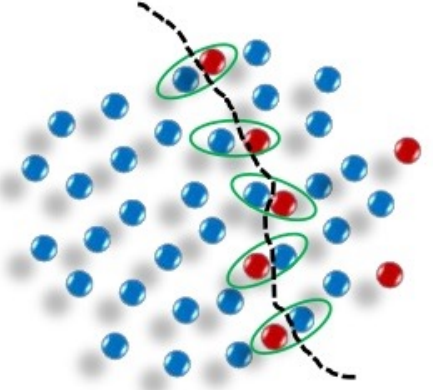
\includegraphics[width=0.5\textwidth]{./img/Preprocessing/tomek.png}
      \caption{Tomek Link}
      \label{fig:tomeklink}
\end{figure}
\section{Features Reduction}
In molti domini applicativi, i dati possono essere rappresentati da un gran
numero di feature che possono essere ridondanti o non informative. In questi casi
è utile ridurre il numero di feature, in quanto:
\begin{itemize}
      \item Si riduce il tempo di calcolo.
      \item Si riduce il rischio di overfitting.
      \item Si riduce il rumore.
      \item Si migliora la comprensione dei dati.
      \item Si migliora la visualizzazione.
\end{itemize}
Esistono diversi metodi per ridurre il numero di feature:
\begin{itemize}
      \item \textbf{Feature Selection}: si selezionano le feature più informative
            e si eliminano quelle ridondanti.
      \item \textbf{Feature Extraction}: si creano nuove feature a partire da
            quelle esistenti.
\end{itemize}
\begin{figure}
      \centering
      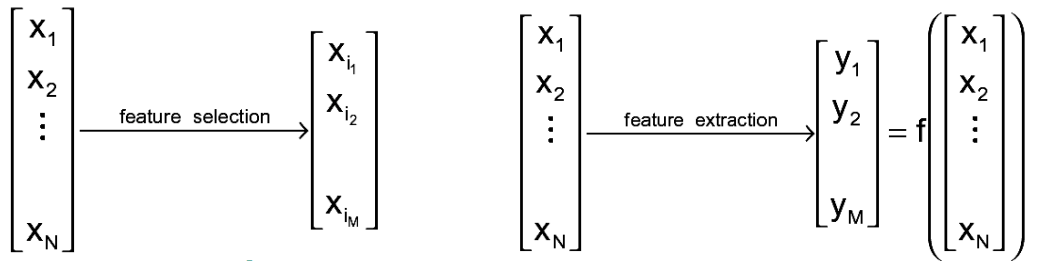
\includegraphics[width=0.5\textwidth]{./img/Preprocessing/features.png}
      \caption{Feature Reduction}
      \label{fig:feature_reduction}
\end{figure}
\subsection{Feature Reduction}
La \textbf{Feature reduction} è un processo che consiste nel selezionare una
funzione $f(x): \mathbb{R}^N \to \mathbb{R}^M$ tale che $M < N$. Questo
significa che si passa da uno spazio di dimensione $N$ a uno spazio di dimensione
$M$. Lo scopo di tale funzione è quello di mantenere il più possibile il
contenuto informativo delle feature originali.

Una funzione ottimale $f$ è quella che permette di non aumentare la probabilità
di errori.

Un esempio di questa funzione è la \textbf{PCA} (\textbf{Principal Component
      Analysis}). Questa funzione permette di proiettare i dati in uno spazio di
dimensione minore, mantenendo il più possibile il contenuto informativo.
\subsection{Feature Selection}
La \textbf{Feature Selection} è un processo che consiste nel selezionare un
sottoinsieme delle feature originali. Dato un insieme di feature $F = \{f_1, f_2,
      \ldots, f_N\}$, si vuole trovare un sottoinsieme $F' \subseteq F$ tale che
$|F'| < |F|$ e che abbia un contenuto informativo simile a $F$.

Esistono diversi metodi per la selezione delle feature:
\begin{itemize}
      \item \textbf{Filter Methods}: si basano su misure statistiche per valutare
            l'importanza delle feature. Questi metodi sono indipendenti dal
            classificatore. Per applicare questo metodo è necessario definire
            una strategia con cui cercare le feature più importanti. Si possono
            utilizzare due strategie:
            \begin{itemize}
                  \item Ricerca esaustiva: se vogliamo passare da $m$ features a
                        $n$ features allora significa controllare il contenuto informativo
                        di ogni sottoinsieme di $n$ feature delle $m$ di partenza. Quindi
                        significa controllare un totale di $\left(\begin{array}{c}
                                    m \\n
                              \end{array}\right) $ sottoinsiemi (esplosione combinatoria).
                  \item Ricerca euristica: si utilizzano delle euristiche per
                        evitare di effettuare una ricerca esaustiva tra tutti i
                        sottoinsiemi (tempi ridotti ma meno qualità nelle feature).
            \end{itemize}
            Solitamente questo metodo viene utilizzato attraverso delle funzioni
            di ranking che permettono di valutare l'importanza delle feature in
            base a misure statistiche, maggiore è il ranking e maggiore sarà
            la qualità della feature. Un esempio di funzione di ranking è la
            \textbf{Information Gain}.
            Il problema di questo metodo è che non tiene conto delle relazioni tra
            le feature. Una soluzione a questo problema è quella di usare
            \textbf{Correlation-based Feature Selection} dove controllo $\left(\begin{array}{c}
                              m \\2
                        \end{array}\right) $ sottoinsiemi.
      \item \textbf{Wrapper Methods}: si basano sull'uso di un classificatore per
            valutare l'importanza delle feature, ovvero la portenza predittiva.
            Questi metodi sono dipendenti dal
            classificatore che viene considerato come una \textit{black box}.

            \begin{figure}[!ht]
                  \centering
                  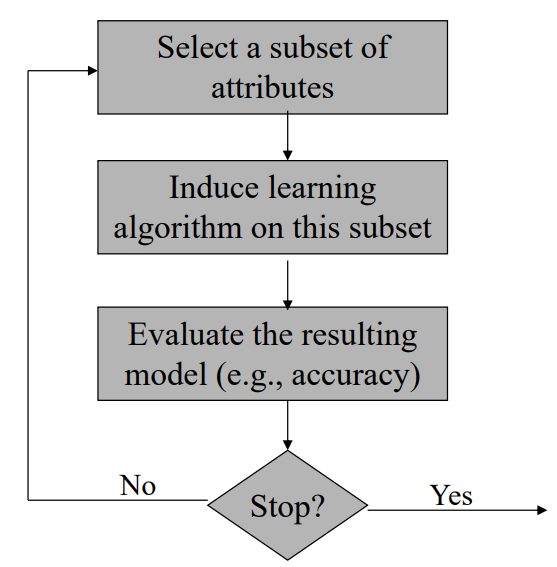
\includegraphics[width=0.5\textwidth]{./img/Preprocessing/wrapper.png}
                  \caption{Wrapper Methods}
                  \label{fig:wrapper}
            \end{figure}
            
            Il problema di questo metodo è che è molto costoso in termini di
            computazione. Si possono utilizzare due strategie:
            \begin{itemize}
                  \item \textbf{Forward Selection}: si parte da un sottoinsieme
                        vuoto e si aggiungono le feature una alla volta in base
                        alla loro importanza.
                  \item \textbf{Backward Elimination}: si parte da un sottoinsieme
                        completo e si eliminano le feature una alla volta in base
                        alla loro importanza.
            \end{itemize}
\end{itemize}

La \textbf{Correlation-based Feature Selection} è un metodo che permette di
selezionare le feature in base alla loro correlazione. Per questo metodo un
buon sottoinsieme di feature è quello in cui le feature sono altamente correlate
con la classe e poco correlate con le altre.
\begin{equation}
      M_s = \frac{k \cdot \overline{r_cf}}{\sqrt{k + k \cdot (k - 1) \cdot \overline{r_ff}}}
\end{equation}
dove $k$ rappresenta il numero di feature nel subset $S$, $\overline{r_cf}$ è la
media delle correlazioni tra le feature e la classe e $\overline{r_ff}$ è la media
delle correlazioni tra le feature.

Spesso i due metodi vengono utilizzati insieme, in quanto il primo permette di
selezionare le feature più importanti, mentre il secondo permette di valutare
l'importanza delle feature in base al classificatore.